\RequirePackage{fix-cm}

\documentclass[smallcondensed]{svjour3}     
\smartqed  
%
\usepackage{graphicx}
%
\usepackage{mathptmx}      % use Times fonts if available on your TeX system
%
\usepackage[utf8]{inputenc}
\usepackage{bm}
\usepackage{amssymb,amsmath}
\usepackage{topcapt,booktabs}
\usepackage{tikz}
\usepackage{pgfplots} 
\pgfplotsset{compat=newest}

\usetikzlibrary{positioning}

\newcommand{\abs}[1]{\lvert#1\rvert}
\newcommand{\floor}{\mathop{\textrm{floor}}\nolimits}
	
\journalname{Formal Methods in System Design}

\begin{document}

\title{Formal Verification of Transcendental Fixed and Floating Point Algorithms using an Automatic Theorem Prover
}
\titlerunning{Transcendental Verification using Theorem Prover}   
\authorrunning{Samuel Coward}
\author{Samuel Coward, Lawrence Paulson, Theo Drane and Emiliano Morini
}
\institute{S.Coward \at
              Faculty of Mathematics, University of Cambridge\\
              \email{src68@cam.ac.uk}   
           \and
           L.Paulson \at
           Computer Laboratory, University of Cambridge\\
	\email{lp15@cam.ac.uk}
    \and
    T.Drane \at
    Cadence Design Systems\\
    \email{theo@cadence.com}
    \and
    E.Morini \at
    Cadence Design Systems\\
    \email{emiliano@cadence.com}
}
\date{Received: date / Accepted: date}
% The correct dates will be entered by the editor


\maketitle

\begin{abstract}
We present a method for formal verification of transcendental hardware algorithms that scales to higher precision without suffering an exponential growth in runtimes. A class of implementations using piecewise polynomial approximation to compute the result is verified using MetiTarski, an automated theorem prover, which verifies a range of inputs for each call. The method was applied to commercial implementations from Cadence Design Systems with significant runtime gains over exhaustive testing methods. It was successful in proving that the expected accuracy of one implementation was overly optimistic.
\keywords{MetiTarski\and transcendental functions \and floating point algorithms \and hardware implementation}
% \PACS{PACS code1 \and PACS code2 \and more}
% \subclass{MSC code1 \and MSC code2 \and more}
\end{abstract}

\section{Introduction}
\label{intro}
Formal verification of floating point operations is becoming ever more challenging as hardware designs reach levels of complexity only previously seen in software. Its importance in industry is well known, exemplified by the Pentium floating point division bug \cite{pratt1995anatomy}. The bulk of this research was conducted during a project at Cadence Design Systems. Building upon this, we present a new approach to the verification of floating point transcendental algorithms. This technique should be viable for verifying high precision algorithms, as our findings suggest that runtimes will not rise exponentially with the precision.  Our experiments cover implementations of logarithms; however, the methodology can also be applied to a wide range of algorithms. 

Traditional techniques rely on exhaustive testing of all inputs to verify such algorithms, but this can be resource intensive, perhaps prohibitively so. The MPFR library is a C library for multiple-precision floating point computations with correct rounding \cite{fousse2007mpfr}, and is widely used as a reference for many verification tasks. For example, some of the industrial implementations presented here were verified by comparing the outputs to the MPFR library. We shall see that the methodology used in this paper performs more efficiently in particular cases. 


The paper will focus on implementations of transcendental functions in hardware that rely on piecewise polynomial approximations. In floating point arithmetic, the upper most portion of the input mantissa is passed to a lookup table which outputs a number of coefficients. The remainder of the input is then used to compute a polynomial approximation to the exact result. Scaling to handle the exponent is often computed in a separate section of the code. Such an approach is easy to verify using the methodology described in this paper, but will hold for any implementation where it is possible to abstract an underlying mathematical model that can be expressed as a system of inequalities for verification purposes.

To produce the required proofs we use MetiTarski~\cite{akbarpour2010metitarski}, an automatic theorem prover for real valued analytical functions such as cosine and logarithm. It's a combination of a resolution theorem prover and a decision procedure for the theory of real closed fields, which together allow it to prove polynomial inequalities. The inbuilt axioms are primarily upper and lower bounds on a set of supported functions. These are obtained from their Taylor or continued fraction expansions, for example
$$\frac{1}{2} \leq x \leq 1 \implies \frac{x-1}{x} \leq \ln(x) \leq \frac{3x^2-4x+1}{2x^2}$$\newline

Conjectures are passed to MetiTarski as a set of inequalities which are transformed by replacing any special function by an appropriate bound. Typically proofs are found in a few seconds \cite{akbarpour2009applications}, but if MetiTarski is unable to prove a conjecture it does not mean that the conjecture is false. For verification it is important that MetiTarski produces machine readable proofs that include algebraic simplification, decision procedure calls, and resolution rules \cite{denman2009formal}. MetiTarski is unique among automated theorem provers in supporting high precision approximations to transcendental functions such as logarithm, cosine, and sine. Our initial research inspired a new enhancement to MetiTarski, and this paper contains the first application of this latest update. It is expected that this enhancement will simplify the verification procedure utilising this methodology and also reduce runtimes with some further development. 


\section{Numerical Algorithms in Hardware}
\label{Num algos}

We present a method to verify designs that rely on making piecewise polynomial approximations to transcendental functions \cite{tang1991table,strollo2011elementary,pineiro2005high}. The input to the function is typically in floating point format \cite{goldberg1991every} which stores a number as $(-1)^{s} \times 2^{e-b} \times 1.\textit{significand}$. In IEEE 754 standard single precision, $s$ is a single bit representing the sign, the exponent $e$ is an 8 bit integer, the bias $b$ is a constant equal to 127, and the significand is 23 bits long. The class of designs verified in this paper are variants on the following high level description. They employ a $k$ bit lookup table and a degree $m$ polynomial approximation:
\begin{enumerate}
\item The top $k$ bits of the significand are passed to a lookup table that outputs some coefficients $a_0,...,a_m$.
\item The lower $23-k$ bits of the significand, say $x$, are used to compute\newline $a_0+a_1x+...+a_mx^m$.
\item A scaling step is computed to account for the exponent.
\end{enumerate} 
Step 3 will vary depending upon the function to be implemented. For example, an algorithm computing logarithm base 2 will simply involve a series of adders. This type of algorithm is typical for computing transcendental functions, evaluating the result with no iteration or convergence test.

The verification methodology described here could be generalised to a wider class of algorithms, for which it is possible to reduce the verification to checking a system of inequalities. 


\section{Verification Methodology}
\label{Method}
Given a hardware implementation of a transcendental function following the template above, we obtain an abstraction that is verifiable using MetiTarski. If the top $k$ bits of the significand are passed to a lookup table, for a fixed 8-bit exponent and sign bit, we reduce the verification problem to $2^k$ calls to MetiTarski. Therefore, the  full verification over all inputs is reduced to 
just $2^{k+8+1}$ MetiTarski conjectures to be proven. In some cases, verification over all such inputs is not necessary: a bespoke hand proof may be able to confirm the correctness of the results for exponent scalings. Of course, most verification tasks use massively parallel processing to reduce the runtimes. Similar methods may be used to reduce the runtimes in our approach, as the conjectures passed to MetiTarski are independent of each other. In nearly all commercial implementations, $k$ is relatively small as lookup tables require a large amount of space on a chip. Assuming that our interpolation coefficients are stored in a file, and we can express the problem as a set of inequalities, the procedure follows the same basic outline.


\begin{quotation}
\textbf{Procedure Outline:}
\begin{enumerate}
\item Write a template problem for the inequalities to be proven, with placeholders for all the relevant interpolation coefficients and upper bit values.
\item Use a wrapper script to read the coefficients and replace them in the template problem to generate the full set of MetiTarski problems.
\item Run the Perl script that accompanies MetiTarski to test all of the problems.
\item Refine error modeling on problems that are not proven.
\item Exhaustively test regions where MetiTarski was unsuccessful.
\end{enumerate}  
\end{quotation}

To demonstrate the methodology we analyse a toy implementation for computing the natural logarithm based on the outline above. The implementation takes as an input an 8 bit integer $x_0x_1...x_7$ and outputs an approximation to $\ln(1.x_0...x_7)$. The top four bits, $x_0..x_3$, are passed to a lookup table that returns the 10 bit interpolation coefficients \textit{a, b, c}. Writing $x=0.x_0...x_7$, the approximation generated is,
$$ \overline{\ln(1+x)}=c + bx +ax^2 $$

This example is designed to be simple to show the underlying principles of the verification methodology. Later we shall adapt it to be more relevant to industrial implementations. In this case, the implementation is accurate to $2^{-10}$:
$$\abs{\ln(1+x)-\overline{\ln(1+x)}} <2^{-10} \qquad (x= 0.x_0...x_7) $$
This can easily be verified using exhaustive testing as the input space is just $2^8$. MetiTarski is able to exactly model this implementation with no errors. We generate a total of 16 problems for MetiTarski to prove, that correspond to the values of the upper 4 bits of the input which determine the interpolation coefficients. For example, the template MetiTarski problem for upper bits, $y=0.x_0...x_3$ and $X$ the value of the lower bits, is
$$ 0\le X \le 2^{-4}-2^{-8} \implies \abs{\ln(1+y+X)-(c+b(y+X)+a(y+X)^2)} $$

Following the outline above with this template problem, all 16 problems are generated and the Perl script automates the MetiTarski calls. Therefore, the only manual input required is to produce the template problem. MetiTarski is able to provide proofs for all of these problems with a total runtime of 5.3 seconds and no more than 0.3 seconds is spent on any one proof. Of course, on such a small input space, exhaustive search is quicker by several orders of magnitude, taking less than a tenth of a second. However, as we shall see, our technique does not suffer from exponentially increasing runtimes as we increase the precision of the implementation.

With this basic understanding of the methodology, we shall make the toy implementation more realistic. Commercial hardware engineers have constraints on area and performance targets to meet, so they apply techniques to reduce the resource requirements. One of these is to truncate bits throughout the algorithm, reducing the number of adders required. This generally improves the performance but typically with some cost to the accuracy of the approximation. In our implementation, we choose appropriate terms to truncate in order to more closely replicate commercial algorithms. The new implementation returns an approximation of the form 
$$ \overline{\ln(1+x)}=c + 2^{-8} \lfloor{b(x_0...x_7)} \rfloor +a(0.x_0...x_5)^2 $$

\noindent In this case, the approximation is accurate to $2^{-7}$: 
\[ 
\abs{\ln(1+x)-\overline{\ln(1+x)}} <2^{-7} \qquad (x= 0.x_0...x_7) \]
This can easily be checked using exhaustive testing, but notice that the implementation uses bit truncations on the first and second order terms. This should mean that the algorithm returns an answer more quickly than the previous method. However, since MetiTarski has no understanding of the integers, such non-analytic functions are are difficult to model. Inspired by this research, we have explored the addition of support for a floor function. MetiTarski understands functions via axioms that give upper and lower bounds, and in the case of the floor function we simply have $x-1< \floor(x)\le x$. It should be noted that this bound is poor when the inputs under investigation are close to 1, for example MetiTarski will fail to prove $\floor(0.5)\geq 0$.
However, for the toy model and other examples investigated in this paper, such a bound is sufficient to verify the function to the same precision that can be verified via exhaustive testing. Therefore, using this function, it is possible to produce a MetiTarski conjecture. We now allow X to be the integer value of the bottom 4 bits and y the integer value of the top 4 bits, which determine the coefficients \textit{a, b, c} as before:
\[
0\le X \le 15 \implies \abs{\ln(1+2^{-4}y+2^{-8}X) - M_1\_\ln(1+x)} <2^{-7}
\]
where $$M_1\_\ln(1+x)=c+2^{-8}\floor(b(X+2^{4}y))+2^{-12}a(\floor(2^{-2}X+2^{2}y))^2$$

An alternative method to model the errors arising from such bit manipulations in the hardware implementations is to include additional error variables in place of the floor function. These techniques were explored before support for the floor function was included, so we can compare both methodologies. Modeling our updated implementation using error variables rather than the floor function yields a MetiTarski problem of the form
\begin{multline*}
	\qquad 0\le X \le 15 \; \land \; 0\le \epsilon_1<1\; \land \; 0\le \epsilon_2<1 \\
	\implies \abs{\ln(1+2^{-4}y+2^{-8}X) - M_2\_\ln(1+x,\epsilon_1,\epsilon_2)} < 2^{-7}\qquad
\end{multline*}
where
$$M_2\_\ln(1+x,\epsilon_1,\epsilon_2)=c+2^{-8}(b(X+2^{4}y)-\epsilon_1)+2^{-12}a((2^{-2}X+2^{2}y)-\epsilon_2)^2$$.

Surprisingly, for this particular problem, using additional error variables rather than the floor function had minimal impact on the overall runtime for the 16 problems. This was unexpected: MetiTarski runtimes can be doubly exponential in the number of variables, an inherent limitation of the decision procedures on which it relies. However, the floor function is a recent addition to MetiTarski and we may be able to improve its performance by fine-tuning its heuristic parameters, which at present are at default values. On industrial implementations, it was necessary to combine manually error variables and estimate an upper bound on these. This was often challenging: some of the error variables can be highly correlated. The floor function has the potential to make the process of generating a template problem significantly simpler. Unfortunately, for the main part of this work, the floor function was not supported and error variables were the only available option.
\begin{figure}
\centering
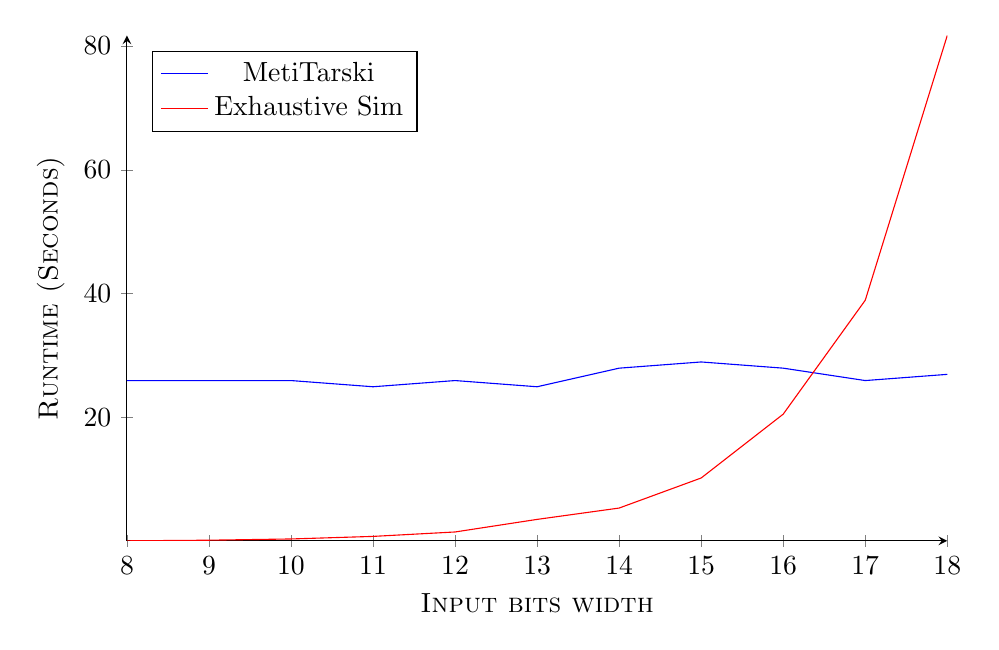
\begin{tikzpicture}
\begin{axis}[
    axis lines = left,
    xlabel = \textsc{Input bits width},
    ylabel = \textsc{Runtime (Seconds)},
    legend pos=north west,height=80mm, width=120mm]

\addplot[
    color=blue,
    ]
    coordinates {(8 ,26)(9 ,26)(10,26)(11,25)(12,26)(13,25)(14,28)(15,29)(16,28)(17,26)(18,27)   };
    \addlegendentry{MetiTarski}
\addplot[color=red,
        ]
        coordinates{(8 ,0.14548254013061523 )
(9 ,0.24578046798706055 )(10,0.4463155269622803  )
(11,0.8605005741119385  )(12,1.574721336364746   )
(13,3.603602409362793   )(14,5.432856559753418)
(15,10.283031702041626)(16,20.580944299697876)
(17,38.95604610443115)(18,81.67475938796997)

 };
        \addlegendentry{Exhaustive Sim}
\end{axis}
\end{tikzpicture}

\caption{A graph demonstrating the runtime comparison of the competing verification procedures on implementations of growing precisions, results obtained running on a single core. \label{runtime_graph}
}
\end{figure}
To see why this technique is powerful, we extend the implementation above to larger input spaces. The approximation is essentially the same, using the same coefficients and lookup table, but our input now may be 10 bits rather than 8 bits, for example. Figure \ref{runtime_graph} compares the runtimes of our methodology and exhaustive testing as the input space grows. Notably, the MetiTarski method has roughly constant runtimes, as we expect: MetiTarski is an analytic tool, so increasing the space of discrete inputs only minimally alters the MetiTarski problems. Conversely, exhaustive testing runtimes suffer from exponential growth in the number of bits of the input. Of course, if the size of the lookup table increases, this will affect the MetiTarski runtimes as the number of problems will grow exponentially. In the results that follow there is still a significant gain.

Even if MetiTarski is only able to prove a subset of the problems passed to it, then the range of the input space upon which we need to do exhaustive testing is reduced. In the following section we shall demonstrate a situation where this technique would have been relevant. 

\section{Applications and Discussion}
\label{Apps}
We present some results from applying this methodology to the verification of several larger commercial implementations. For intellectual property reasons it is not possible to describe the particular implementations in detail but the runtime results can be found in Table \ref{result} and demonstrate that the technique has real world relevance. 

The single precision floating point $\log_2$ was a release candidate for Cadence Design Systems. It takes as inputs 32 bit floating point numbers and outputs in the same format. This was the first test case studied using the MetiTarski verification methodology and previously the implementation had been checked using a basic benchmarking tool. Through our investigations, we discovered that the expected accuracy of the implementation was breached for a small input region. First using the methodology described above inputs in the region $[0.5,2)$ were verified. Since exponent scaling for $\log_2$ simply involves adding the exponent to the approximation made on the $1.\textit{significand}$ component, a bespoke and simple hand proof was sufficient to complete the verification. However the proof identified a region in which the  claimed accuracy may be breached and exhaustive testing on this region identified a large number of counterexamples. For the purpose of validating our methodology, we exhaustively tested all inputs: as predicted, everywhere but in this narrow region the implementation met its accuracy claim.

The second implementation in Table \ref{result} is an experimental test case generated primarily to analyse how the MetiTarski method performed on higher precision algorithms. It takes as input a fixed point number with 8 bits before the decimal place and 24 bits after. Therefore, the total number of possible inputs is $2^{32}$, but it is a higher precision algorithm and is more accurate as it makes use of a larger lookup table.
\begin{table}[h]
\caption{Verification runtime results for industrial implementations of logarithm base 2, results obtained running on a single core}
\label{result}     
\begin{tabular}{lll}
\hline\noalign{\smallskip}
Design & Floating point $\log_2$ & Fixed point 8.24 $\log_2$    \\

\noalign{\smallskip}\hline\noalign{\smallskip}

 Input Region Verified& $[0.5,2)$ & $[1,2) $ \\ 
 MetiTarski Problems & 128 & 512 \\
 MetiTarski Time (mins.) &  7 & 4 \\ 
 Exhaustive Test Time (mins.) & 42 & 53 \\
\noalign{\smallskip}\hline
\end{tabular}
\end{table}
We see that the speedup achieved by MetiTarski is significant on the floating point logarithm. Notably it was even greater for the higher precision experimental implementation. Such an observation suggests that this methodology could be viable for verification of higher precision hardware, where traditional exhaustive techniques are infeasible. 

In addition to the results above, we applied our technique to a more complex algorithm, which had aleady been formally verified. Here we were only able to prove a subset of the problems, so were able to reduce the space on which exhaustive testing was necessary. Through this experience we discovered a significant shortcoming of the approach. Generating the initial template problem is a non-trivial task. The verification engineer needs a deep understanding of the design implementation in order to model the errors correctly. A simpler error model may be used initially to establish whether the algorithm is correct to a higher error rate, but to obtain a full proof, several refinements of the model might be required. This aspect of the technique becomes time consuming when trying to verify more involved algorithms. For example, a sequence of \textbf{if} and \textbf{else if} statements, which can be found in some hardware algorithms, are difficult to model using this technique. By comparison, exhaustive testing is far simpler to implement: it requires only knowledge of the output and the correct answer, which we may reasonably assume we have given the existence of the MPFR library. This fact currently limits the circumstances under which our method is useful. 

\section{Related work}
\label{Related}
John Harrison conducted some of the earliest work on floating point algorithm verification via theorem proving, using the HOL proof assistant~\cite{harrison1997floating}. Such an approach is labour intensive and not easily adaptable to changes in the algorithm: for example an increase in the input bit width would require a large portion of the work to be done again. Note however that Harrison's proofs are more detailed and refer to specific features of the IEEE floating point standard, such as the various available rounding modes. 

An important problem for verification will be the interplay of floating point and bit level operations, common in real code. For example, computing $2^n$ in double precision can be done by shifting $n+1023$ left by 52 bits \cite{mine2012abstract}, which is computationally efficient. Such techniques make verification more challenging, particularly in the context of high precision transcendental functions \cite{lee2016verifying}. 

For verification of small floating point functions, the Gappa tool \cite{de2006assisted,boldo2009combining} has been tested and is still being developed. Gappa uses interval arithmetic in order to prove conjectures whilst MetiTarski relies on cylindrical algebraic decomposition to generate proofs. Both methods are valid; interval arithmetic is weaker but considerably more efficient. Hopefully this study may lead to a comparison of the two approaches to verification in the future.

\section{Conclusion}
\label{Conclusion}
We have successfully verified a variety of fixed and floating point logarithm implementations using the MetiTarski theorem prover.
We have also identified a bug in an algorithm that was close to production. Most interesting are the performance results, which provide strong evidence to suggest that this technique will be viable in the future when higher precision algorithms are developed. For a set of algorithms following a basic outline, it is possible to automate the whole verification procedure after the initial template and wrapper scripts are written. In such a setting the technique is quite powerful. However, for algorithms not following a standard format, the verification process requires significantly more manual effort by a skilled verification engineer than alternative methods. For some cases, the approach may be unsuccessful if the algorithm uses techniques we can't model using MetiTarski. 

It should be noted that this is just a first investigation into this technique and further research may yield new methods for modelling more complex algorithms. Further development of MetiTarski could enhance its power or simplify the process, as the introduction of the floor function has already done. A possible extension is the use of a binary chop applied to the input region of each problem, which may allow the engineer to further reduce the input space on which exhaustive testing is necessary. For implementations that follow a standard model and particularly bespoke higher precision implementations, the methodology shows promise.

\begin{acknowledgements}
We would like to thank Mathew Eaton and Ran Zmigrod for helpful contributions during the initial investigations. Much of the preliminary work for this paper was done at Cadence Design Systems, who were supportive throughout. 
\end{acknowledgements}
\bibliographystyle{unsrt}   
\bibliography{bibliography.bib}  



\end{document}


